%! Author = Stepan Oskin
%! Date = 2019-07-22

% Preamble
\documentclass[11pt]{article}
\usepackage{graphicx}
\usepackage{subcaption}

% Packages

% Document
\begin{document}

    \title{Relational databases \\
    Description of methodology \\
    Based on a course offered by DataCamp \\
    \textit{Introduction to Relational Databases}\cite{Grossenbacher2019} \\
    and other sources}

    \author{Stepan Oskin}

    \maketitle

    \begin{abstract}
        A relational database models real life entities, such as universities and university professors, by storing them in tables.
        The idea of a database is to push data into a certain structure \textemdash a pre-defined model \textemdash where you can enforce data types, relationships, and other rules.
        Each table must contain data from a single entity type.
        This reduces redundancy by storing entities only once.
        A database can then be used to model relationships between entities and to preserve data quality through such concepts as constraints, keys, and referential integrity.
        SQL, or Structured Query Language, can be used for querying, as well as building and maintaining databases.
    \end{abstract}

    \section{Relational Database} \label{sec:rdb}

    A relational database models real life entities, such as universities, organizations, and university professors, by storing them in tables.
    Each table must contain data from a single entity type (\textit{e.g.}, universities, organizations, university professors, \textit{etc.})
    This reduces redundancy by storing entities only once \textemdash for example, there only needs to be one row of data containing details of a certain university.
    Lastly, a database can be used to model relationships between entities.
    For instance, a professor could be involved with multiple organizations within a university, while an organization may include many professors.

    An example of data organized with redundancy in attributes and without redundancy is presented in the two entity-relationship diagrams on figure~\ref{fig:ent_rel_diag}.
    The diagram on the left (fig.\ref{fig:with_redun}) models only one entity type \textemdash \texttt{university\_professors}.
    However, this table actually holds multiple entity types, and thus causes redundancy in entries, as the same professor and university can be present in multiple rows, for example, in cases where the professor is involved with multiple organizations within the same university.
    The updated entity-relationship model (fig.\ref{fig:without_redun}) would be better suited in this case.
    It represents three entity types \textemdash "professors", "universities", and "organizations" \textemdash in their own tables, with respective attributes.
    This reduces redundancy, as professors, unlike in fig.~\ref{fig:with_redun}, need to be stored only once.
    For each professor, the respective university is denoted through the \texttt{university\_shortname} attribute.

    \vspace{5mm}

    Characteristics of a relational database:
    \begin{itemize}
        \item real-life \textit{entities} become \textit{tables}
        \item reduced redundancy
        \item data integrity by \textit{relationships}
    \end{itemize}

    \begin{figure}[hbt!]
        \centering
        \begin{subfigure}[t]{.48\textwidth}
            \centering
            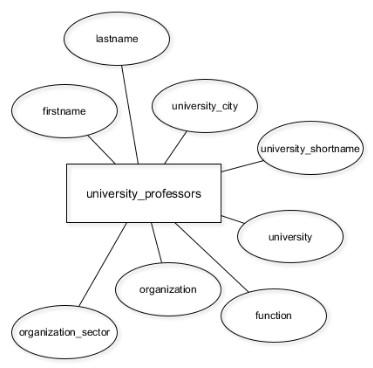
\includegraphics[width=\columnwidth,trim=4 4 4 4,clip]{img/ent_rel_diag1.png}
            \caption{with redundancy}
            \label{fig:with_redun}
        \end{subfigure}
        ~ %add desired spacing between images, e. g. ~, \quad, \qquad, \hfill etc.
        %(or a blank line to force the subfigure onto a new line)
        \begin{subfigure}[t]{.48\textwidth}
            \centering
            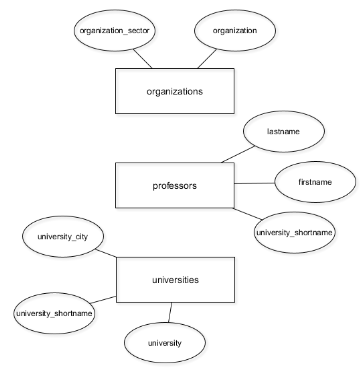
\includegraphics[width=\columnwidth,trim=4 4 4 4,clip]{img/ent_rel_diag2.png}
            \caption{without redundancy}
            \label{fig:without_redun}
        \end{subfigure}
        \caption{These two entity-relationship diagrams show examples of organizing data with redundancy in attributes (fig.~\ref{fig:with_redun}), and without redundancy (fig.~\ref{fig:without_redun}).
        Squares denote the so-called entity types, and circles connected to these denote attributes (or columns).}
        \label{fig:ent_rel_diag}
    \end{figure}


    \section{Integrity constraints} \label{sec:constraints}

    The idea of a database is to push data into a certain structure \textemdash a pre-defined model \textemdash where you can enforce data types, relationships, and other rules.
    Generally, these rules are called \textbf{integrity constraints}, although different names exist.

    \vspace{5mm}

    Integrity constraints can roughly be divided into 3 types:

    \begin{enumerate}
        \item \textbf{Attribute constraints}, \textit{e.g.}, data types on columns
        \item \textbf{Key constraints}, \textit{e.g.,} primary keys
        \item \textbf{Referential integrity constraints}, \textit{e.g.,} enforced through foreign keys
    \end{enumerate}

    Benefits of using constraints include:

    \begin{itemize}
        \item Constraints press data into a certain structure
        \item Constraints help with consistency, and thus data quality (\textit{e.g.,} by ensuring that the certain format is followed during manual or automated data entry)
        \item Data quality is a business advantage / data science prerequisite
        \item Enforcing constraints is difficult, but database management systems (\textit{e.g.,} PostgreSQL) help
    \end{itemize}

    \subsection{Attribute constraints} \label{subsec:att_constr}

    In its simplest form, attribute constraints are data types that can be specified for each column in a table.
    There are basic data types for numbers, such as \texttt{bigint}, or strings of characters, such as \texttt{character varying}.
    There are also more high-level data types, such as \texttt{cidr}, which can be used for IP addresses.
    Implementing such a data type on a column would disallow anything that doesn't fit the structure of an IP .

    Data types also restrict possible SQL operations on the stored data.
    For example, it is impossible to calculate a product from an \texttt{integer} and a \texttt{text} column.
    In case if a column with data type \texttt{text} contains numbers that need to be used in calculations, on-the-fly type conversions, or \textbf{type casts} can be used to allow the required operation using the \texttt{CAST} function in SQL .
    Examples of some data types from \textit{PostgreSQL documentation}\cite{ThePostgreSQLGlobalDevelopmentGroup2019} are presented on figure~\ref{fig:dtypes}.

    \begin{figure}[hbt!]
        \centering
        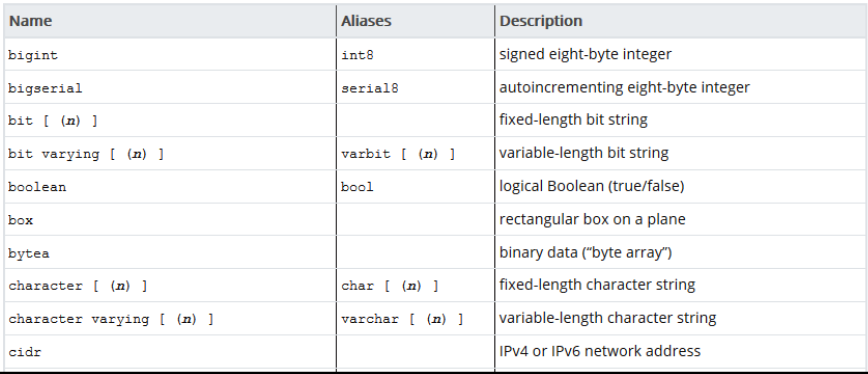
\includegraphics[width=1\linewidth,trim=1 1 1 1,clip]{img/dtypes.png}
        \caption{Beginning of the list of all data types from PostgreSQL documentation\cite{ThePostgreSQLGlobalDevelopmentGroup2019}.}
        \label{fig:dtypes}
    \end{figure}

    \subsubsection{Data types} \label{subsubsec:dtypes}

    Working with data types can be straightforward in a database management system such as PostgreSQL .
    As said before, data types are attribute constraints and are therefore implemented for a single column of a table.
    They define the so-called \textit{domain of values} in a column, that means, what form these values can take \textemdash and what not.
    Therefore, they also define what operations are possible with the values in the column.
    Through this, consistent storage is enforced, so a street number will always be an actual number, and a postal code will always have exactly 6 characters, according to the defined conventions.
    This greatly helps with data quality.

    To sum up, data types in a database management system are:

    \begin{itemize}
        \item Enforced on columns (\textit{i.e.,} attributes)
        \item Define the so-called \textit{domain} of a column
        \item Define which operations are possible
        \item Enforce consistent storage of values
    \end{itemize}

    Most common data types in PostgreSQL include:

    \begin{itemize}
        \item \texttt{text}: character string of any length
        \item \texttt{varchar [ (n) ]}: a maximum of \texttt{n} characters
        \item \texttt{char [ (n) ]}: a fixed-length string of \texttt{n} characters
        \item \texttt{boolean}: can only take three states, \textit{e.g.,} \texttt{TRUE}, \texttt{FALSE}, and \texttt{NULL} (unknown)
        \item \texttt{date}, \texttt{time}, and \texttt{timestamp}: various formats for date and time calcualtions
        \item \texttt{numeric}: arbitrary precision numbers, \textit{e.g.,} 3.1457
        \item \texttt{integer}: whole numbers in the range of -2'147'483'648 and +2'147'483'647
        \item \texttt{bigint}: whole numbers in a larger range
    \end{itemize}

    These data types are specific to PostgreSQL, but appear in many other database management systems as well, and they mostly conform to the SQL standard.

    \subsubsection{The \texttt{not-null} constraint} \label{subsubsec:not_null}

    Another type of attribute constraints are the \textbf{not-null} constraints.
    The not-null constraint disallows any \texttt{NULL} values on a given column.
    This must hold true for the existing state of the database, as well as for the future state.
    Therefore, we can only specify a not-null constraint on a column that doesn't hold any \texttt{NULL} values yet.
    And, it won't be possible to insert any null values in the future.

    There is no clear definition of what do \texttt{NULL} values actually mean.
    \texttt{NULL} can mean a couple of things, for example, that the value is unknown, or does not exist at all.
    It can also be possible that the value does not apply to the column.
    One important takeaway is that two \texttt{NULL} values must not have the same meaning.
    This also means that comparing \texttt{NULL} with \texttt{NULL} always results in a \texttt{FALSE} value.

    To sum up, the not-null constraints:

    \begin{itemize}
        \item Disallow \texttt{NULL} values in a certain column.
        \item Must hold true for the current state
        \item Must hold true for any future state
        \item \texttt{NULL} can mean different things: does not exist, does not apply, missing, \textit{etc.}
        \item Therefore, \texttt{NULL~!=~NULL}
    \end{itemize}

    \subsubsection{The \texttt{unique} constraint} \label{subsubsec:unique}

    The unique constraint on a column makes sure that there are no duplicates in a column.
    So, any given value in a column can only exist once.
    This makes sense in cases where storing values more than once leads to unnecessary redundancy.
    However, it does not make sense in cases where it is expected that values might repeat.
    Just as with the not-null constraint, we can add a unique constraint if the column does not have any duplicates before we apply it.
    Making sure that a column contains only unique values is a prerequisite for turning them into \textit{primary keys}

    To sum up, unique constraint:

    \begin{itemize}
        \item Disallows duplicate values in a column
        \item Must hold true for the current state
        \item Must hold true for any future state
        \item Is a prerequisite for turning the column into a primary key
    \end{itemize}

    \subsection{Key constraints} \label{subsec:keys}

    Key constraints are a very important concept in database systems.
    Attribute constraints discussed in subsection~\ref{subsec:att_constr}, such as data types, not-null, and unique constraints, do not change the structure of the database model.
    Key constraints, such as primary keys, do make a change in the model and, thus, are reflected in the entity-relationship diagram.
    Attributes corresponding to keys are denoted by underlying the attribute names.

    Typically, a database table has an attribute, or a combination of multiple attributes, whose values are unique across the whole table.
    Such attributes identify a record in this table uniquely.
    Normally, a table, as a whole, only contains unique records, meaning that the combination of all attributes is a key in itself.
    However, it's not called a key, but a \textbf{superkey},  if attributes from that combination can be removed, and the attributes still uniquely identify records.
    If all possible attributes have been removed, but the records are still uniquely identifiable by the remaining attributes, we speak of a minimal superkey.
    This is the actual key.
    So a key is always minimal.
    Minimal superkeys are also called candidate keys.
    In the end, there can only be one key for a table, which has to be chosen from candidates.

    To sum up the information about keys, in a database:

    \begin{itemize}
        \item A key is an attribute/multiple attributes that identify a record uniquely
        \item As long as attributes can be removed: \textbf{superkey}
        \item If no more attributes can be removed: minimal superkey, or \textbf{key}
        \item Minimal superkeys are also called candidate keys
        \item Only one candidate key can be the \textit{chosen} key
    \end{itemize}

    \subsubsection{Primary keys} \label{subsubsec:primary_keys}

    Primary keys are one of the most important concepts in database design.
    Almost every database table should have a primary key, chosen from a set of candidate keys.
    The main purpose of a primary key is to uniquely identify records in a table, and ideally, primary keys consist from as few columns as possible.
    For instance, this makes it easier to reference these records from other tables.
    Primary keys need to be defined on columns that don't accept duplicate or null values.
    Lastly, primary key constraints are time invariant, meaning that they must hold for the current data in the table \textemdash but also for any future data a table might hold.
    It is therefore wise to choose columns where values will always be unique and not null.

    A table can have one and only one primary key.
    It is a good practice to add a primary key to every table.
    When we add a primary key to a table, PostgreSQL creates a unique B-tree index on the column or a group of columns used to define the primary key.\cite{ThePostgreSQLGlobalDevelopmentGroup2019a}

    To sum up the information about primary keys, in a database:

    \begin{itemize}
        \item One primary key per database table, chosen from candidate keys
        \item Uniquely identifies records, \textit{e.g.,} for referencing in other tables
        \item Unique and not-null constraints both apply
        \item Primary keys are time-invariant and therefore must be chosen wisely
        \item Ideally, primary keys consist from as few columns as possible
        \item It is a good practice to add a primary key to every table.
    \end{itemize}

    \subsubsection{Surrogate keys} \label{subsubsec:surrogate_keys}

    Surrogate keys are sort of an artificial primary key.
    In other words, they are not based on a native column in the data, but on a column that just exists for the sake of having a primary key.
    There are several reasons for creating an artificial surrogate key.
    As mentioned in subsection~\ref{subsubsec:primary_keys}, a primary key is ideally constructed from as few columns as possible.
    Secondly, a primary key of the record should never change over time.
    If we define an artificial primary key, ideally consisting of a unique number or string, we can be sure that this number stays the same for each record.
    Other attributes might change, but the primary key always has the same value for a given record.

    There is a special data type in PostgreSQL that allows the addition of auto-incrementing numbers to an existing table: the \texttt{serial} type.
    It is specified just like any other data type.
    Once we add a column with a \texttt{serial} type, all the records in the table would be numbered.
    Whenever a new record is added to the table, it will automatically be given a number that does not exist yet.
    There are similar data types in other database management systems, like MySQL .
    Also, if we try to specify an ID that already exists, the primary key constraint will prevent us from doing so.

    Another strategy for creating a surrogate key is to combine two existing columns into a new one.
    The \texttt{CONCAT} function glues together the values of two or more existing columns.
    After creating a new column and updating it with concatenated values, we can turn the new column into a surrogate primary key.

    To sum up the information about surrogate keys, in a database:

    \begin{itemize}
        \item Primary keys should be built from as few columns as possible
        \item Primary keys should never change over time
        \item When this conditions are not met by native columns in a table, surrogate keys can be used as artificial primary keys
        \item For example, using the \texttt{serial} data type in PostgreSQL would assign a unique, non-null, auto-incrementing id to each record in a table
        \item Alternatively, surrogate keys can be created by concatenating several existing columns using the \texttt{CONCAT} function.
    \end{itemize}

    \subsection{Referential integrity constraints} \label{subsec:ref_integrity}

    Now, we will model the relationships between professors and universities.
    As we know, in our database each professor works for a university.
    In the ER diagram (presented on figure~\ref{fig:fk}), this is drawn with a rhombus.
    The small numbers specify the cardinality of the relationship: a professor works for at most one university, while a university can have any number of professors working for it \textemdash even zero.
    Such relationships are implemented with \textbf{foreign keys}.

    Foreign keys are designated columns that point to a primary key of another table.
    There are some restrictions for foreign keys.
    First, the domain and the data type of a foreign key must be the same as one of the primary key to which it is linked to.
    Secondly, only foreign key values that exist as values in the primary key of the referenced table are allowed.
    This is the actual foreign key constraint, also called \textbf{referential integrity}.
    Lastly, a foreign key is not necessarily an actual key, because duplicates and \texttt{NULL} values are allowed.

    \begin{figure}[hbt!]
        \centering
        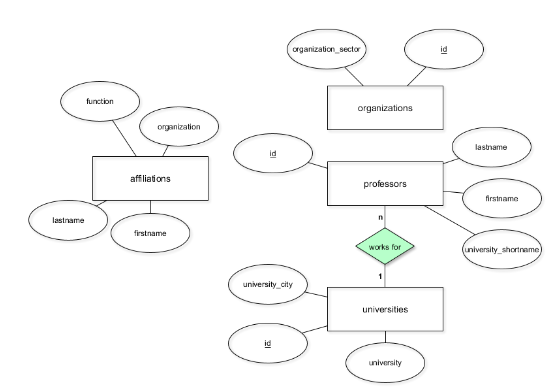
\includegraphics[width=1\linewidth,trim=1 1 1 1,clip]{img/fk.png}
        \caption{In the entity-relationship (ER) diagram, relationships between entities are drawn with a rhombus.
        The small numbers specify the cardinality of the relationship: in this database, a professor works for at most one university, while a university can have any number of professors working for it \textemdash even zero.}
        \label{fig:fk}
    \end{figure}

    To sum up the information about foreign keys, in a database:

    \begin{itemize}
        \item A foreign key (FK) points to a primary key (PK) of another table
        \item Domain of FK must be equal to domain of PK
        \item Each value of FK must exist in PK of the other table (FK constraint, or \textbf{referential integrity})
        \item FKs are not actual keys \textemdash \texttt{NULL} and duplicate values are allowed
    \end{itemize}

    \section{\texttt{information\_schema} database} \label{sec:info_schema}

    \texttt{information\_schema} database is available by default in PostgreSQL and presents a \textit{meta database} that holds information about a relational database in PostgreSQL .
    \texttt{information\_schema} is not PostgreSQL specific, and is also available in other database management systems, such as MySQL or SQL Server.
    The \texttt{information\_schema} database holds various information in different tables, for example, in a \texttt{tables} or \texttt{columns} tables.

    \subsection{Querying \texttt{information\_schema} using \texttt{SELECT * FROM} syntax} \label{subsec:info_schema_q}

    SQL, or \textbf{Structured Query Language}, can be used for querying, as well as building and maintaining databases.
    \texttt{information\_schema} has multiple tables you can query with the known \texttt{SELECT * FROM} syntax:

    \begin{itemize}
        \item \texttt{tables}: information about all tables in your current database
        \item \texttt{columns}: information about all columns in all of the tables in your current database
        \item \ldots
    \end{itemize}

    \vspace{5mm}

    \textbf{Example}: get information on all table names in the current database, while limiting your query to the 'public' \texttt{table\_schema}.

    \vspace{5mm}

    \texttt{-- Query the right table in information\_schema \\
    SELECT table\_name \\
    FROM information\_schema.tables \\
    -- Specify the correct table\_schema value \\
    WHERE table\_schema = 'public';}

    \vspace{5mm}

    \textbf{Example}: get information on all column names in a particular table, while limiting your query to the 'public' \texttt{table\_schema}.

    \vspace{5mm}

    \texttt{-- Query the right table in information\_schema to get columns \\
    SELECT column\_name, data\_type \\
    FROM information\_schema.columns \\
    WHERE table\_name = 'nhl\_draft' AND table\_schema = 'public';}

    \medskip
    \bibliography{rdbms}
    \bibliographystyle{ieeetr}

\end{document}